\documentclass[9pt,aspectratio=169]{beamer}

% --- Theme ---
\usetheme{Singapore}
\setbeamertemplate{navigation symbols}{}   % no icons
\setbeamertemplate{mini frames}{}          % no dots in headline
\setbeamercovered{transparent}

% --- Grayscale colors ---
\definecolor{PelloGrayDark}{RGB}{60,60,60}
\definecolor{PelloGray}{RGB}{120,120,120}
\definecolor{PelloGrayLight}{RGB}{235,235,235}
\definecolor{PelloGrayUltraLight}{RGB}{248,248,248}

\usecolortheme[named=PelloGrayDark]{structure}

% --- Blocks ---
\setbeamertemplate{blocks}[rounded][shadow=false]
\setbeamercolor{block title}{fg=white,bg=PelloGrayDark}
\setbeamercolor{block body}{fg=black,bg=PelloGrayLight}
\setbeamercolor{block title example}{fg=white,bg=PelloGrayDark}
\setbeamercolor{block body example}{fg=black,bg=PelloGrayLight}
\setbeamercolor{section in head/foot}{fg=PelloGray,bg=PelloGrayLight}
\setbeamercolor{subsection in head/foot}{fg=PelloGray,bg=PelloGrayLight}
\setbeamercolor{frametitle}{fg=black}

% --- Itemize bullets (optional; keep if you like the style) ---
\setbeamertemplate{itemize item}{\raisebox{0.2em}{\scalebox{.6}{$\bullet$}}}
\setbeamertemplate{itemize subitem}{\raisebox{0.2em}{\scalebox{1}{$-$}}}

% --- Footer: frame numbers ---
\makeatletter
\setbeamertemplate{footline}{%
  \hfill\usebeamerfont{footline}\insertframenumber/\inserttotalframenumber\hspace{1em}\vspace{2pt}
}
\makeatother

% --- Minimal packages (add more only when needed) ---
\usepackage[english]{babel}
\usepackage[T1]{fontenc}
\usepackage[utf8]{inputenc}
\usepackage{graphicx}
\usepackage{tikz}
\usepackage{booktabs}
\usepackage{makecell} % for jumping lines within cells in tables.
\usepackage{multirow}
\usepackage{amsmath}
\usepackage{hyperref}
\hypersetup{colorlinks,linkcolor=,urlcolor=blue}
\usepackage{comment}
\usepackage{listings}
\lstset{
  language=R,
  basicstyle=\ttfamily\footnotesize,
  keywordstyle=\color{blue},
  commentstyle=\color{green!50!black},
  stringstyle=\color{red},
  frame=single,
  showstringspaces=false
}
\linespread{1.7}   % 1.0 = normal, 1.2–1.5 common
\AtBeginEnvironment{lstlisting}{\linespread{1}\selectfont} % keep code listings single-spaced

% --- Meta ---
\title{Applied Economics}
\subtitle{Introduction}
\author{Pello Aspuru}
%\institute{University of Vienna}
\date{Winter 2026/2027}

% --- Title page spacing + bottom-left author/date ---
\setbeamertemplate{title page}{
  \vspace{8em}
  \begin{center}
	{\usebeamerfont{title}\inserttitle\par}
  	\vspace{1.5em} % <-- increase title–subtitle gap
  {\usebeamerfont{subtitle}\insertsubtitle\par}
  \end{center}
  \vspace{4em}
  \begin{flushleft}
    {\usebeamerfont{author}\insertauthor\par}
    {\usebeamerfont{date}\insertdate}
  \end{flushleft}
}

\begin{document}

% Title slide without headline/footer
{
  \setbeamertemplate{headline}{}
  \setbeamertemplate{footline}{}
  \begin{frame}
    \titlepage
  \end{frame}
}


\section[Course Logistics]{Introduction}

\begin{frame}[fragile]{Welcome to Applied Economics}

%Lectures
%\begin{itemize}
%    \item Wednesday (040178-1) 16:45-18:15, PC-Seminarraum 5
%    \item Thursday (040178-2)  16:45-18:15, PC-Seminarraum 3 
%\end{itemize}


All course material (including these slides) will be distributed via \textbf{moodle}.

\alert{Prior knowledge at the level of Introductory Econometrics (BA) will be assumed throughout the course.}

%For course structure and deadlines, see the \href{syllabus}{syllabus}

Class participation is highly encouraged, determines 10\% of final grade.

Office hours: by email appointment via pello.aspuru@univie.ac.at

\onslide<2>{
People who signed up online for this class and signed the list today
are considered \textbf{enrolled}.

If you are registered, you will receive a grade!
}
\end{frame}

\begin{frame}{Course Overview}
 \begin{block}{In this Course You Will Learn to...}
\begin{itemize} 
\item Use econometric tools to produce empirical analyses.
\item Learn to interpret, and critically evaluate existing empirical studies.
\item Understand possibilities and limitations of empirical analyses.
\end{itemize}
\end{block}
\end{frame}

\begin{frame}{Course Tools}
\onslide<1->{
\begin{block}{Statistical Software: R and RStudio}
\begin{itemize} 
\item Freely available open source software
\item Active user community providing up-to-date functions \& support
\item Extensive statistical modeling capabilities
\item Relevant for industry jobs
\end{itemize}
\end{block}}

\onslide<2->{
\begin{block}{Auxiliary Software}
\begin{itemize} 
\item Large Language Models (ChatGPT, Claude etc.) to support learning \& coding.
\item Latex for drafting academic-style documents, problem set.
\end{itemize}
\end{block}}

\end{frame}

\begin{frame}{Course Assessment}

\begin{block}{Class Participation (10\%)}
\begin{itemize} 
\item[] Classroom engagement through questions \& comments is encouraged!
\end{itemize}
\end{block}

\begin{block}{Midterm Exam (25\%)}
\begin{itemize}
%\item based on classes, slides, and problem sets
\item[] Preliminary date: November 25th/26th 2026.\\
%\item Preliminary location: TBD.
%\item there will be no resit
\end{itemize}
\end{block}

\onslide<2->{
\begin{block}{Project Presentations (25\%)}
\begin{itemize}
\item Work on the project in groups of up to 3 students, fill in names using the link provided by Moodle.
\item Presentation I (10\%): December 16th/17th 2026.
\item Presentation II (15\%): January 20th/21st 2027.
\end{itemize}
\end{block}

\begin{block}{Final exam (40\%)}
\begin{itemize} 
%\item based on classes, slides, and problem sets
\item[] Date: Wednesday, 27th January 2027. \\
%\item Preliminary location: lecture hall 9, 01.314 Oskar-Morgenstern-Platz 1, OG 1st floor
%\item there will be no resit
\end{itemize}
\end{block}}

%All tasks are compulsory. Missing \textit{any} of them implies failing the course.
\end{frame}

\begin{frame}{Useful Textbooks}
\linespread{1.3}\selectfont % dense slide: tighter line spacing so it fits
  \begin{enumerate}
    \item \textbf{Heiss, F. (2020).} Using R for Introductory Econometrics (2nd edition)\\
    available online: \href{http://urfie.net/readOnline.html}{http://urfie.net/readOnline.html}

    \item \textbf{Hanck, C., Arnold, M., Gerber, A., \& Schmelzer, M. (2023).} Introduction to Econometrics with R\\
    available online: \href{https://www.econometrics-with-r.org/index.html}{https://www.econometrics-with-r.org/index.html}

    \item \textbf{Oswald, F., Viers, V., Villedieu, P., \& Kennedy, G. (2020).}
    Introduction to Econometrics with R. Sciences Po, Department of Economics, Paris, France.\\
    available online: \href{https://scpoecon.github.io/ScPoEconometrics/}{https://scpoecon.github.io/ScPoEconometrics/}.
  \end{enumerate}

  \vspace{0.3cm}
  If you need to read up on theoretical concepts:
  \begin{itemize}
    \item Angrist, J. D., \& Pischke, J.-S. (2008). Mostly Harmless Econometrics. % Princeton University Press.
    \item Wooldridge, J. (2015). Introductory Econometrics: A Modern Approach. % (Sixth edition, student ed.)
    % \item Hill, R. C., Griffiths, W. E., \& Lim, G. C. (2018). Principles of Econometrics (5th ed.)
  \end{itemize}
\end{frame}

\section{Motivation}

\begin{frame}{What is Applied Economics?}
\linespread{1.5}\selectfont % dense slide: tighter line spacing so it fits

\begin{center}
  The use of economic theory and \textbf{data} to answer real-world \textbf{economic} questions.
\end{center}

\begin{itemize}
\onslide<2->{
\item \textcolor{teal}{Test} what economic theory predicts.
\begin{itemize}
\item Theory: a higher minimum wage reduces employment. Do we see this in the data?
\end{itemize}}
\onslide<3->{
\item \textcolor{teal}{Discover} (causal) relationships between economic variables and \alert{quantify} them.
\begin{itemize}
%\item Does more education \textcolor{teal}{increase earnings}? \alert{If so, by how much?}
\item Does immigration \textcolor{teal}{increase unemployment} for locals? \alert{By how much?}
\end{itemize}}
\onslide<4->{
\item \textcolor{teal}{Evaluate and design} policies that achieve the intended objective at the \textbf{lowest possible cost.}
\begin{itemize}
%\item Do job training programmes for the unemployed affect the chance to find a new job?
\item How much money do we need to subsidize public transport to save 1 ton of carbon emissions?
\end{itemize}}
\end{itemize}

\onslide<5->{
\begin{block}{}
  \begin{enumerate}
    \item Gather, clean and combine multiple sources of data $\rightarrow$ Tidy dataset.
    \item Find patterns in the data $\rightarrow$ Data Visualization and Descriptive Statistics.
    \item Apply econometric tools $\rightarrow$ Establish causality and estimate magnitude.
  \end{enumerate}
\end{block}

}

\end{frame}




%\begin{frame}{What We Will Focus on in This Course}
%How to estimate coefficients of the MLR using R?

%When do the coefficients of the MLR reflect actual causal effects of interest?

%How to do statistical inference?

%What are frequently used modern \textit{quasi-experimental methods} and how can we apply them in R? 

%\end{frame}

\begin{comment}
\section{Course Outline}

\begin{frame}[fragile]{Course Outline}
1. Introduction \textit{(Heiss, Sections 1 - 1.4, 1.6)}
 \begin{itemize}
   \item Motivation
    \item Introduction to R
\end{itemize}

2. Revisiting the Multiple Linear Regression Model \\
\textit{(Heiss, 3.1 and 3.3; Wooldridge 3.1--3.2)}
\begin{columns}
    \begin{column}{0.38\linewidth}
    \begin{itemize}
     \item Structure and terminology 
    \item Use for causal analysis  
    \end{itemize} 
    \end{column}
        \begin{column}{0.46\linewidth}
\begin{itemize}
   
    \item Matrix Notation
    \item Deriving the OLS estimator
\end{itemize} 
    \end{column}
\end{columns}

3. Revisiting the Multiple Linear Regression Model II \\
\textit{(Heiss, 6.1 and 7; Wooldridge 3.3 and 5.1-5.2)}
\begin{columns}
    \begin{column}{0.38\linewidth}
    \begin{itemize}
    \item MLR Assumptions 
    \item Properties of the OLS estimator
     \end{itemize} 
    \end{column}
        \begin{column}{0.46\linewidth}
\begin{itemize}
    \item Accommodating nonlinear relationships
\end{itemize}
    \end{column}
\end{columns}
%12 lectures
%PSET due dates
\end{frame}

\begin{frame}[fragile]{Course Outline}
4. - OLS Variance \textit{(Heiss, 3.4, 8.1; Hanck et al. 5.4)} \\ \hspace*{+.27cm} - more R topics: \texttt{ggplot2}, \texttt{for-loops} \textit{(Heiss, 1.9)}

5. Inference I \textit{(Heiss, 4.1-4.2; Wooldridge, Ch. 4.1-4.3)}
    \begin{itemize}
     \item t-Tests, p-values, confidence intervals
    \end{itemize} 
    
6. - Inference II: \textit{(Heiss, 4.3-4.4, 8.1; Wooldridge, Ch. 4.4-4.5)}
\vspace{-0.05cm}
 \begin{itemize}
     \item Multiple Hypothesis Testing
    \end{itemize} 
    \vspace{+0.15cm}

\\ \hspace*{+.275cm} - More R topics: writing own functions    \textit{(Heiss, 1.9.3)}
   
%12 lectures
%PSET due dates
\end{frame}

\begin{frame}[fragile]{Course Outline}
7. Endogeneity  \textit{(Hanck et al. 9-9.2, 9.4)}

8. Instrumental Variable Estimation \textit{(Oswald et al. Ch. 11)}

9. Panel Data methods \textit{(Oswald et al. Ch. 12)}

10. Diff-in-Diff Estimator \textit{(Hanck et al. Ch. 13.4)}

11. Regression Discontinuity Design \textit{(Hanck et al. Ch. 13.4)}
%12 lectures
%PSET due dates
\end{frame}
\end{comment}


\section{Introduction to R}


\begin{frame}{What is R ?}

\begin{itemize}
    \item \textbf{Programming Language} A formal system of rules and symbols that allows humans to write instructions a computer can understand and execute.
    \begin{itemize}
      \item Perfect replicability.
    \end{itemize}
    \item \textbf{R} is a programming language and software environment for\dots
    \begin{itemize}
      \item Data tidying.
      \item Data visualization.
      \item Statistical and econometric analysis.
    \end{itemize}
    \item Install R from \url{https://cran.r-project.org/}
\end{itemize}
\end{frame}

\begin{frame}[fragile]{Basic R Programming Concepts}

\textbf{Code} instructions written in a programming language.

\begin{columns}

\begin{column}{0.6\textwidth}
\begin{itemize}
  \item \textbf{Script} a .R text file with many lines of code.
  \item \textbf{Comment} code lines ignored by the computer, used to explain or annotate your work. Comments start with \#.
  \item \textbf{Object} a piece of information (like a number, or dataset) stored in memory that can be used and modified by your code.
  \item \textbf{Function} a reusable “recipe” that takes some objects, performs a specific task and returns an output.
  %\vspace{0.2cm}
  %\item \textbf{Run} = executing the instructions of the code.
\end{itemize}
\end{column}

\begin{column}{0.4\textwidth}
\begin{lstlisting}[language=R, basicstyle=\ttfamily\tiny]
# This is a comment

# Create object "n"
n <- 100

# Define the function "square()"
square <- function(x) { return(x^2) }

# Run function on object, store as "result"
result <- square(n)

# Print the result in the console
print(result)
\end{lstlisting}
\end{column}
\end{columns}
\end{frame}

\begin{frame}{What is RStudio?}

\begin{itemize}
    \item \textbf{RStudio} a workspace that provides a user-friendly interface to write and run code.
    \item  Install RStudio from \url{https://posit.co/download/rstudio-desktop/}
    \item R Studio interface consists of 4 main windows (panes):
\end{itemize}
\begin{figure}[h]
    \centering
    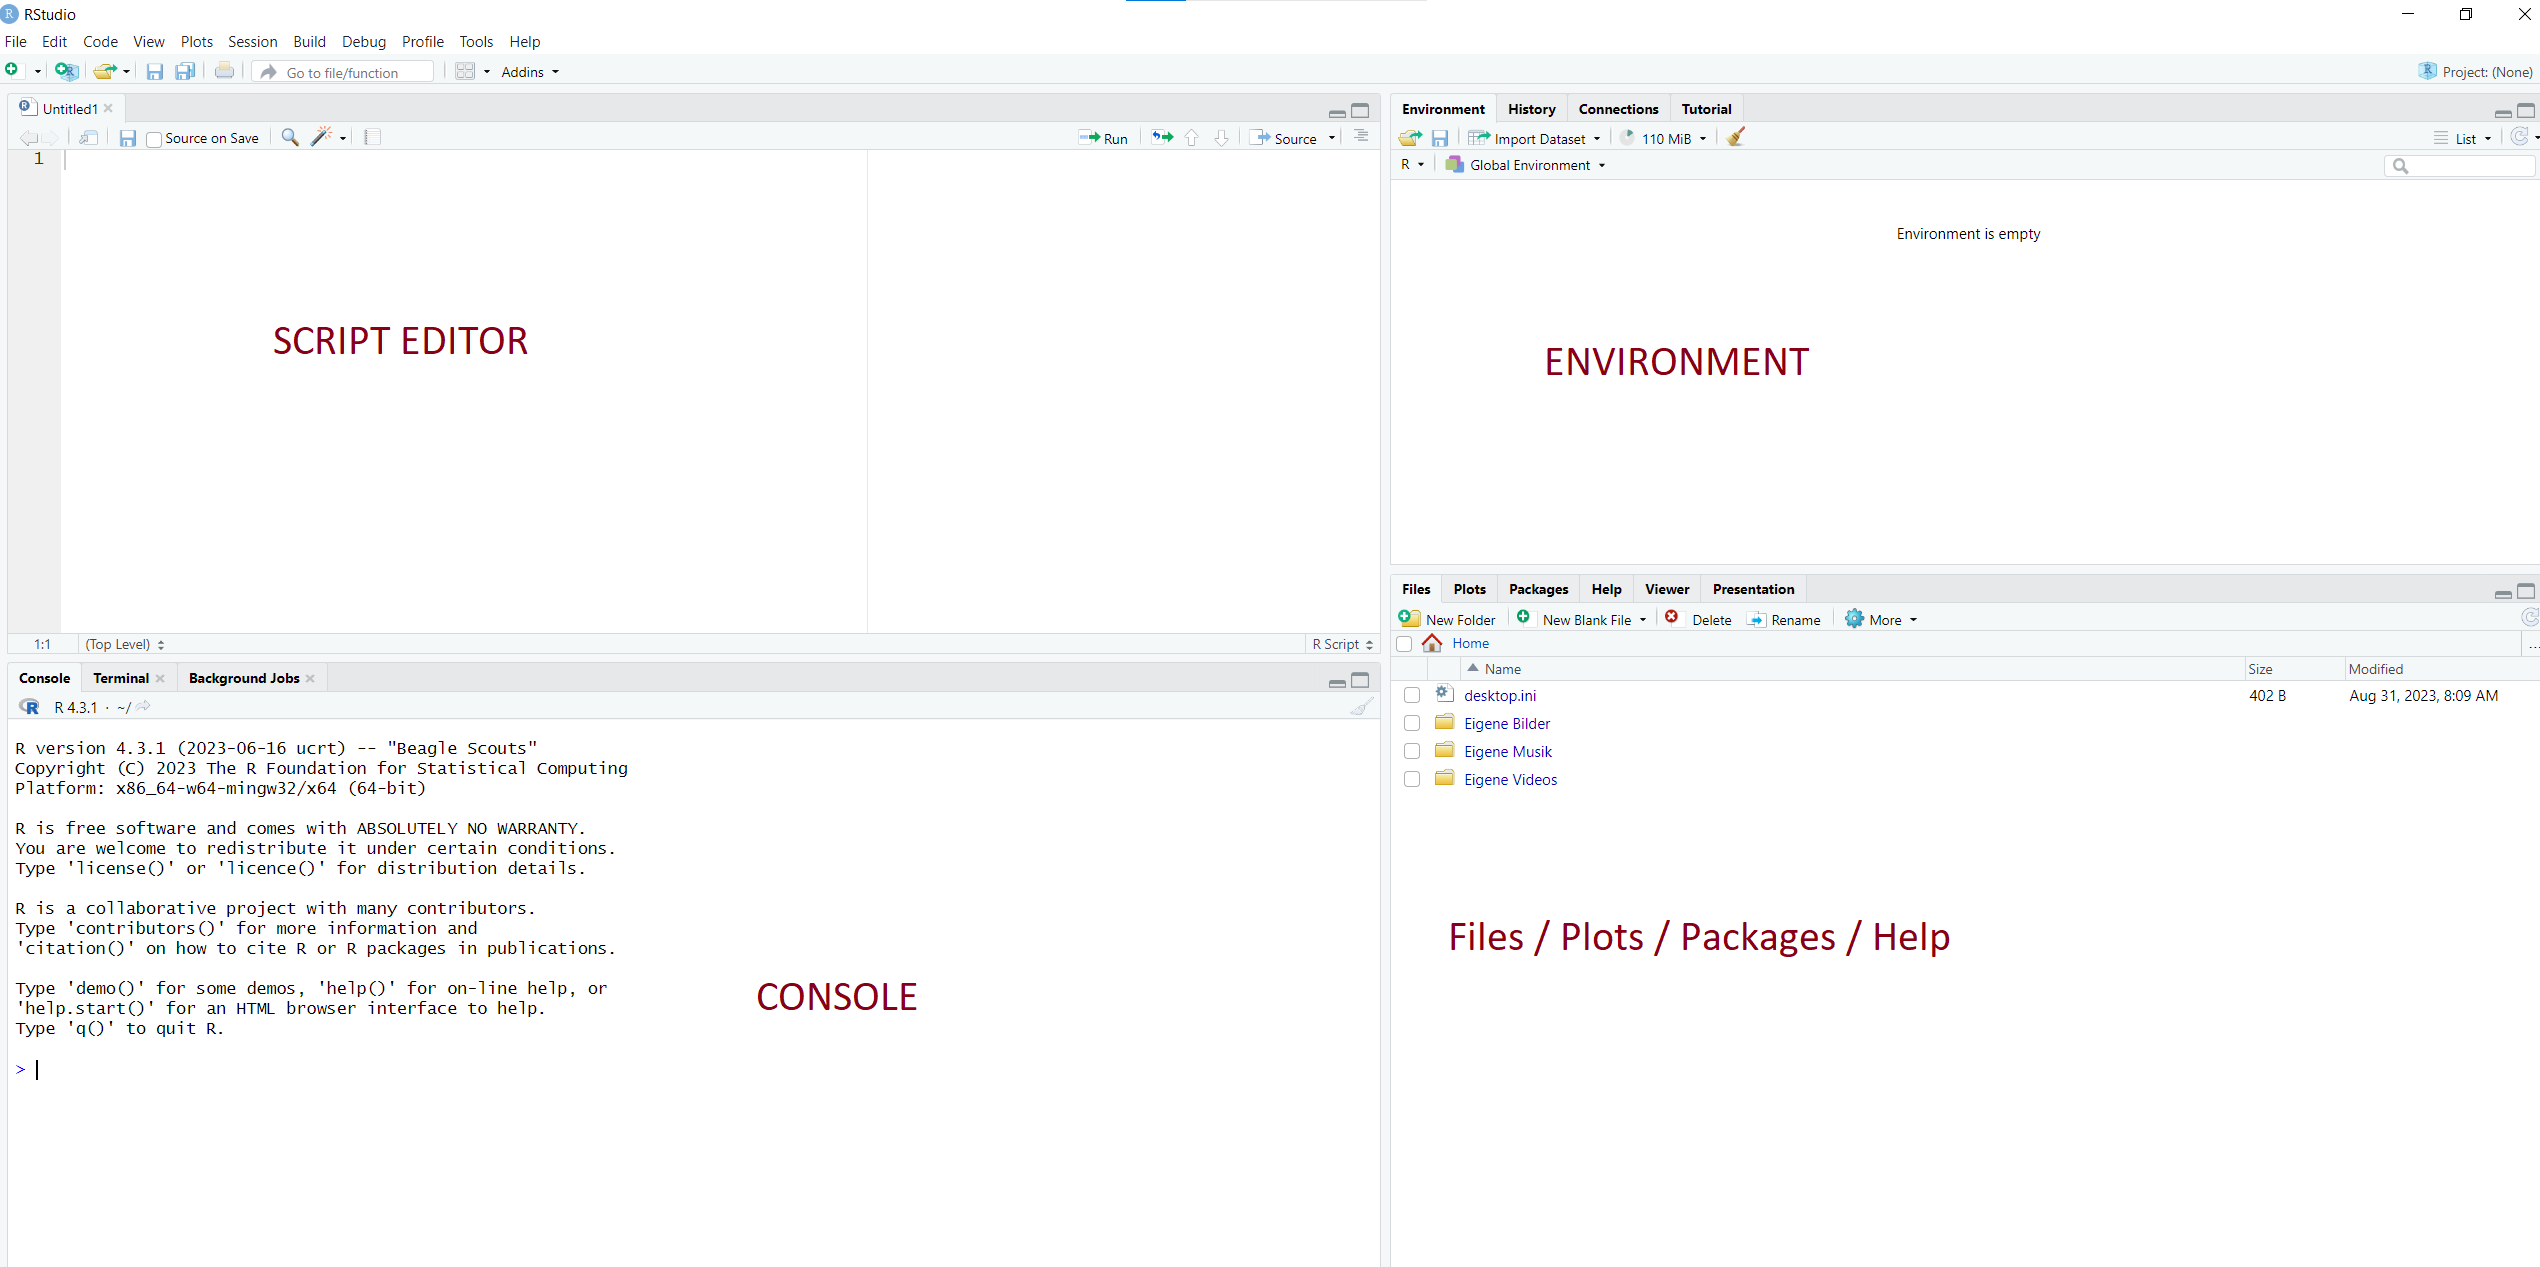
\includegraphics[width=0.6\linewidth]{Rstudio.png}
\end{figure}
\end{frame}

\begin{frame}{RStudio Interface}

% Reserve a fixed vertical space for the text overlays
\begin{overlayarea}{\textwidth}{0.35\textheight}
\begin{enumerate}
  \only<1>{\item[] \textbf{Console}
    \begin{itemize}
      \item Output of your coding and computations appears here (exception: graphs).
      \item It is possible to write code directly into the console.
      \alert{\item Do not use the console to make changes to the data.}
    \end{itemize}}

  \only<2>{\item[] \textbf{Script Editor}
    \begin{itemize}
      \item Open a new R script: click $File \rightarrow New \, File \rightarrow R \, Script$.
      \item Always write your main code in a script: allows you to save and keep track of your work, and to re-run the analysis or make modifications later.
      \item To send the code in your script to the console, click $run$.
    \end{itemize}}

  \only<3>{\item[] \textbf{Environment}
    \begin{itemize}
      \item list of all objects you created
      \item second pane provides $History$ of commands entered into the console
    \end{itemize}}

  \only<4>{\item[] \textbf{Files / Plots / Packages / Help / Viewer window}
    \begin{itemize}
      \item \textit{Plots} you create appear here.
      \item if you search for \textit{Help}, information appears here.
    \end{itemize}}
\end{enumerate}
\end{overlayarea}

\vfill % keeps the image glued to the bottom

\begin{center}
  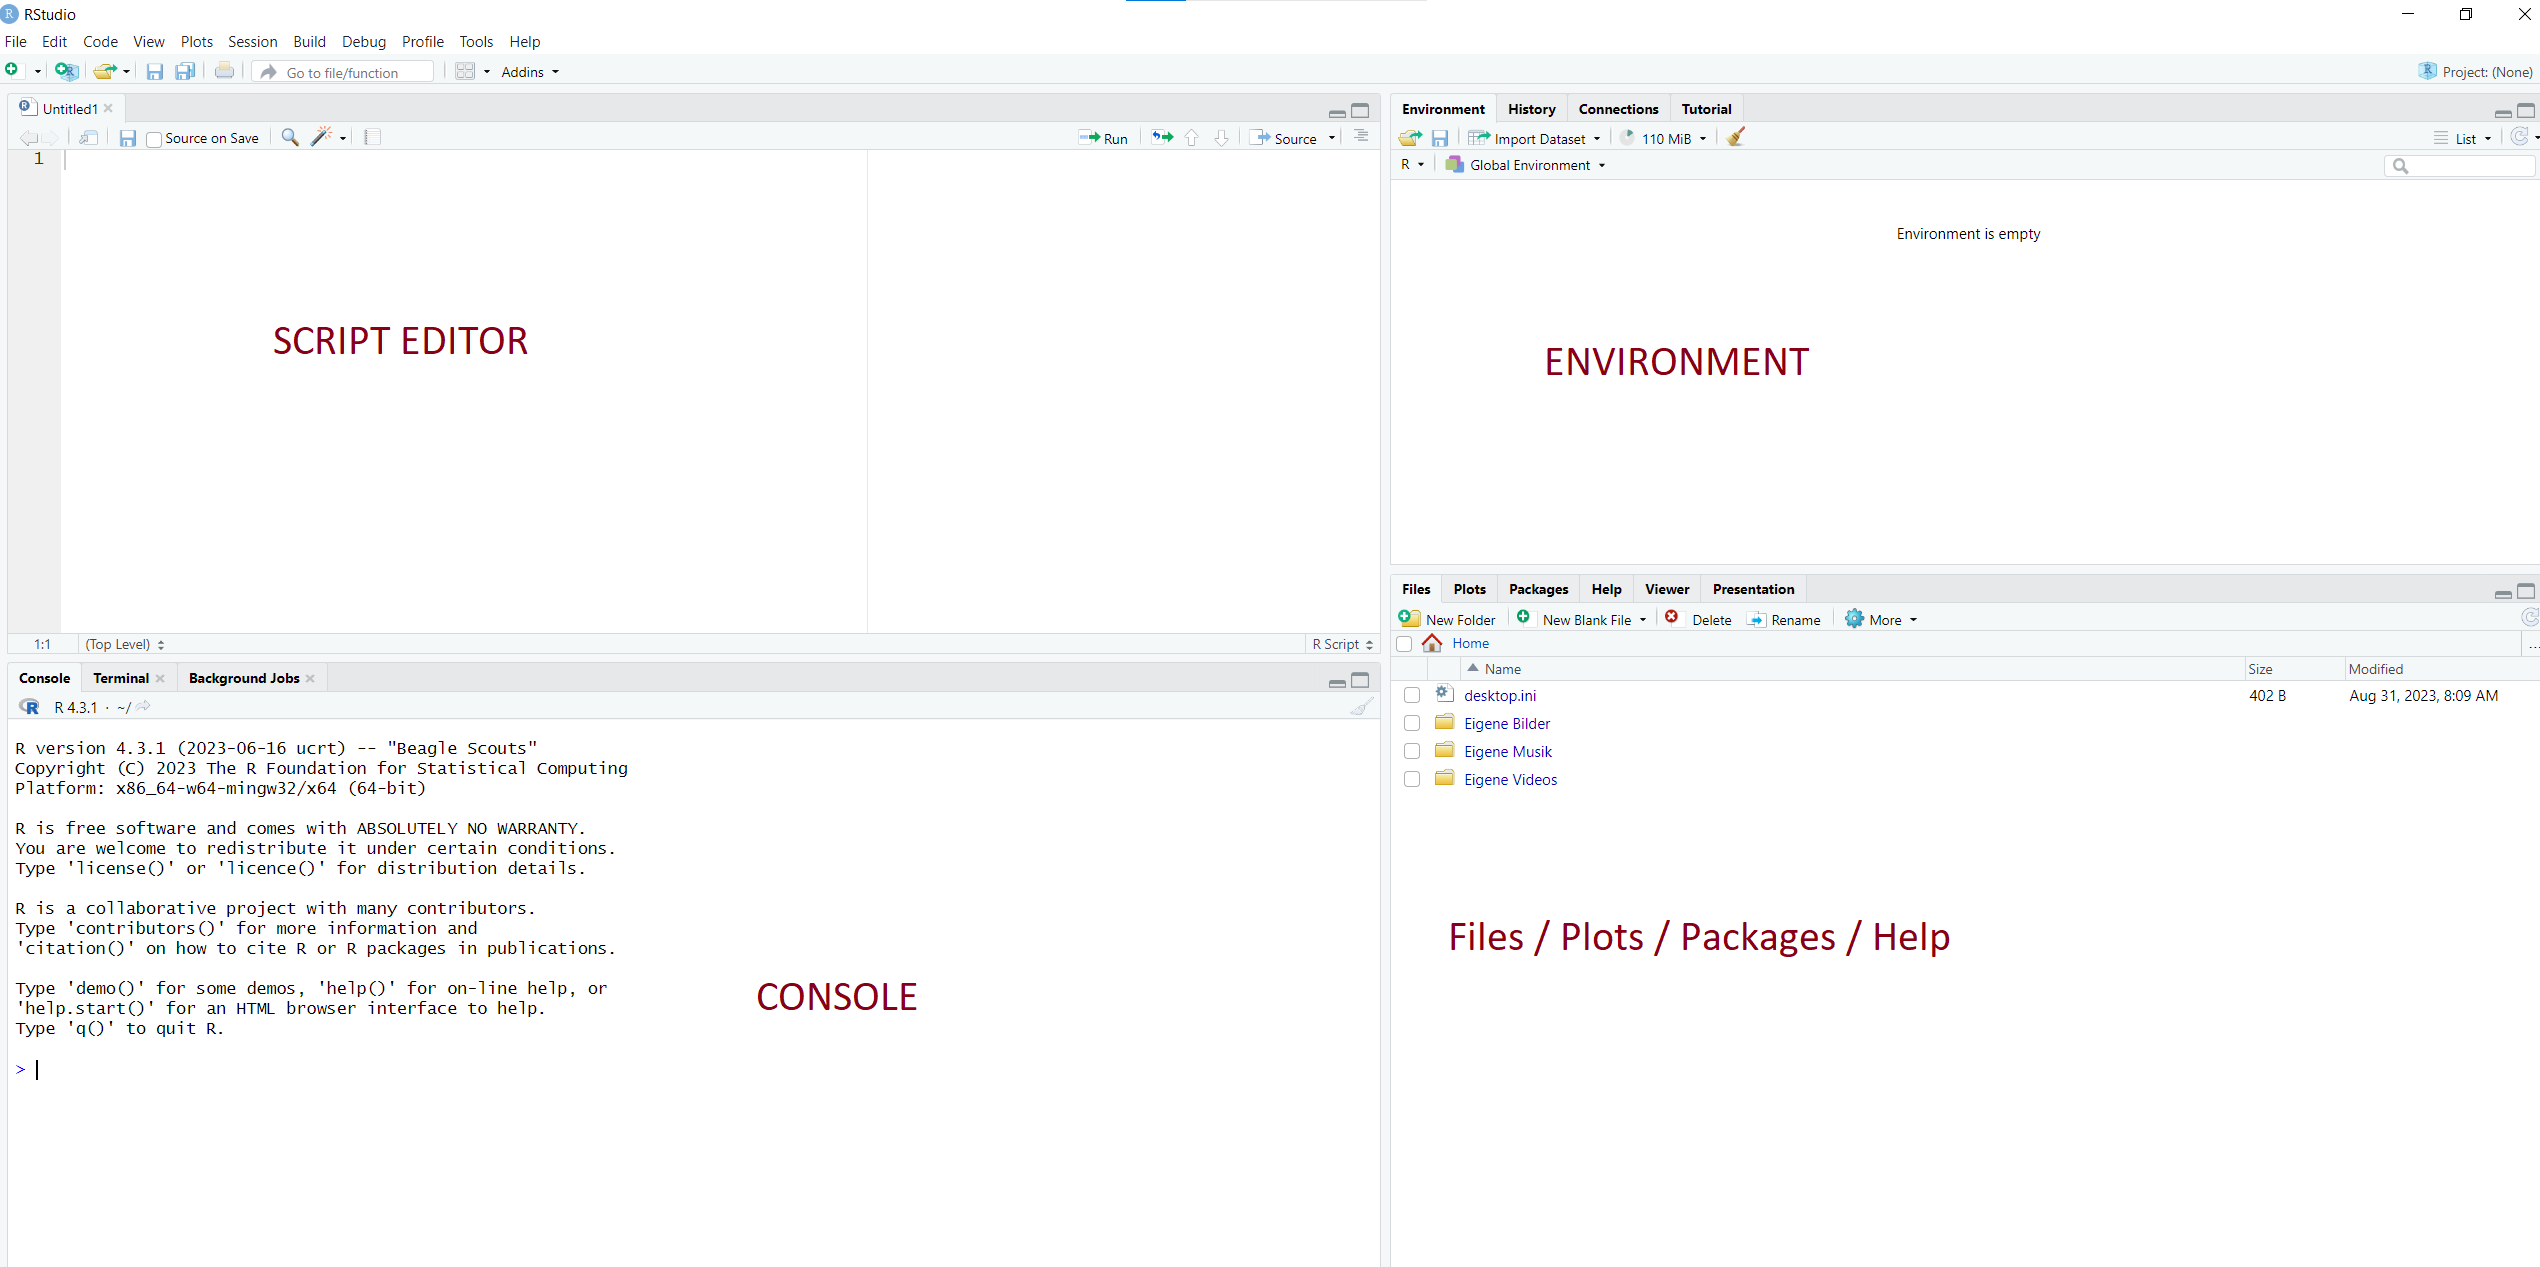
\includegraphics[width=0.45\linewidth]{Rstudio.png}
\end{center}
\end{frame}

\begin{frame}[fragile]{Script Set Up}

\textbf{Working directory} is the default folder on your computer where R reads and saves files, unless you tell it otherwise.

\begin{columns}

\begin{column}{0.6\textwidth}
\onslide<2->{
\begin{itemize}
    \item Comments start with \#: R ignores them.
    \item Create a new folder on your desktop called "AE\_2026" to use as your working directory.
    \item show current working directory {\tt getwd()}
    \item setting new working directory to newly created folder \texttt{setwd("C:/Users/.../AE\_2026")}
    \item list all files in your working directory \texttt{dir()}
\end{itemize}}
\end{column}

\begin{column}{0.4\textwidth}
\begin{lstlisting}[language=R, basicstyle=\ttfamily\tiny]
# This is a comment

# Check current working directory
getwd()

# Set a new working directory.
setwd("C:/Users/YourName/Desktop/AE_2026")

# Verify the change
getwd()

# List files in the working directory
dir()
\end{lstlisting}
\end{column}
\end{columns}
\end{frame}

\begin{frame}[fragile]{Clean the Environment}

\begin{itemize}
  \item Every object you create stays in the \textbf{environment} until you remove it.
  \item Start every script from a clean environment, so that your results do not depend on objects left over from earlier work.
  \item list all objects: \texttt{ls()}; remove all of them: \texttt{rm(list = ls())}
\end{itemize}

\begin{lstlisting}[language=R, basicstyle=\ttfamily\small]
# List all objects in the environment
ls()

# Remove all objects from the environment
rm(list = ls())

# Verify the change
ls()
\end{lstlisting}
\end{frame}


\begin{frame}[fragile]{R Objects}
\textbf{Object} a piece of information (like a number, word, vector, or dataset) stored in memory that can be used and modified by your code.
\pause
\begin{columns}
  \begin{column}{0.5\textwidth}
      \begin{itemize}
          \item create an object: \texttt{object <- ...}
          \item print object to the console: \texttt{object}
          \item identify format using \texttt{str(object)}
          \item get basic information on the object:  \texttt{class(object), dim(object)}
          \item list all objects: \texttt{ls()}
          \item remove an object: \texttt{rm(object)}
      \end{itemize}
  \end{column}
  \begin{column}{0.5\textwidth}
\begin{lstlisting}[language=R, basicstyle=\ttfamily\tiny]
# Create object "n"
n <- 100

# Print the object in the console:
n

# generate vector "age":
age <- sample(18:65, n, replace = TRUE)

# Visualize
age # Print object in console
str(age) # Object type, size
class(age) # Object type
dim(age)
ls() # List all objects
\end{lstlisting}
  \end{column}
\end{columns}

\end{frame}

\begin{frame}[fragile]{Vectors}
\linespread{1.3}\selectfont % dense slide: tighter line spacing so it fits

\textbf{Vector} an ordered sequence of values of the same type (all numbers, or all words).

\begin{columns}
  \begin{column}{0.45\textwidth}
      \begin{itemize}
          \item \texttt{AirPassengers}: built-in dataset with the number of airline passengers (in thousands) in each month from 1949 to 1960.
          \item number of elements: \texttt{length(vector)}
          \pause
          \item access elements by their position, in square brackets: \texttt{vector[...]}
      \end{itemize}
  \end{column}
  \begin{column}{0.55\textwidth}
\begin{lstlisting}[language=R, basicstyle=\ttfamily\scriptsize]
# Three vectors with one value per month
passengers <- as.numeric(AirPassengers)
year       <- as.numeric(floor(time(AirPassengers)))
month      <- as.numeric(cycle(AirPassengers))

length(passengers)     # 144

# Access elements of a vector
passengers[1]          # first element: 112
passengers[1:3]        # elements 1 to 3: 112 118 132
passengers[c(1, 144)]  # first and last: 112 432
\end{lstlisting}
  \end{column}
\end{columns}

\end{frame}

\section{Data Frames}

\begin{frame}[fragile]{From Vectors to Dataframes}
\linespread{1.3}\selectfont % dense slide: tighter line spacing so it fits

Dataframes are two-dimensional objects that store data in a tabular format, with rows and columns:
\begin{itemize}
  \item Rows: units of observation (individuals, years, ...).
  \item Columns: variables (e.g. income, education, GNP, ....) [vectors]
\end{itemize}
\pause
\texttt{data.frame()} puts vectors of the same length side by side as columns; \texttt{head()} prints the first rows:

\begin{columns}[c]
  \begin{column}{0.4\textwidth}
\begin{lstlisting}[language=R, basicstyle=\ttfamily\tiny]
# Create a dataset from the three vectors
df_air <- data.frame(year, month, passengers)
dim(df_air)            # 144 rows, 3 columns
\end{lstlisting}
\begin{lstlisting}[language=R, basicstyle=\ttfamily\tiny]
> head(df_air)
  year month passengers
1 1949     1        112
2 1949     2        118
3 1949     3        132
4 1949     4        129
5 1949     5        121
6 1949     6        135
\end{lstlisting}
  \end{column}
  \begin{column}{0.5\textwidth}
  \centering
  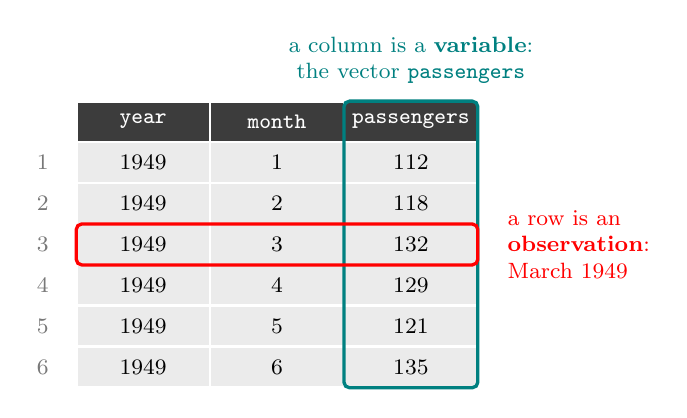
\begin{tikzpicture}[x=1.7cm, y=0.52cm, font=\footnotesize,
    cell/.style={draw=white, line width=1pt, fill=PelloGrayLight, minimum width=1.7cm, minimum height=0.52cm, inner sep=0pt},
    head/.style={cell, fill=PelloGrayDark, text=white, font=\footnotesize\ttfamily}]
    % header
    \node[head] at (0,0) {year};
    \node[head] at (1,0) {month};
    \node[head] at (2,0) {passengers};
    % rows
    \foreach \r/\v in {1/112, 2/118, 3/132, 4/129, 5/121, 6/135} {
      \node[text=PelloGray] at (-0.75,-\r) {\r};
      \node[cell] at (0,-\r) {1949};
      \node[cell] at (1,-\r) {\r};
      \node[cell] at (2,-\r) {\v};
    }
    % one column = one vector
    \draw[teal, line width=1.2pt, rounded corners=2pt] (1.5,0.5) rectangle (2.5,-6.5);
    \node[teal, align=center] at (2,1.5) {a column is a \textbf{variable}:\\ the vector \texttt{passengers}};
    % one row = one observation
    \draw[red, line width=1.2pt, rounded corners=2pt] (-0.5,-2.5) rectangle (2.5,-3.5);
    \node[red, align=left, anchor=west] at (2.65,-3) {a row is an\\ \textbf{observation}:\\ March 1949};
  \end{tikzpicture}
  \end{column}
\end{columns}

\end{frame}


\begin{comment}
  \begin{frame}[fragile]{More Objects}
  The \texttt{sample()} function randomly samples from categorical variables.
  \begin{lstlisting}[language=R, basicstyle=\ttfamily\tiny]
        # More vector objects
        gender   <- sample(c("Male", "Female"), n, replace = TRUE)
        education<- sample(c("High School", "Bachelor","Master", "PhD"), n, replace = TRUE,
                           prob = c(0.4, 0.35, 0.2, 0.05))
 \end{lstlisting}
 \pause
 The \texttt{rnorm()} function randomly samples from a random normal distribution for a certain mean \texttt{mean} and standard deviation \texttt{sd}.
  \begin{lstlisting}[language=R, basicstyle=\ttfamily\tiny]
        income   <- round(rnorm(n, mean = 40000 + 1500*age/10, sd = 8000), 0)
 \end{lstlisting}
 \pause
 The \texttt{ifelse()} function generates a pre-determined outcome when a logical condtion is fulfilled.
  \begin{lstlisting}[language=R, basicstyle=\ttfamily\small]
        employed <- ifelse(income > 35000, 1, 0)
 \end{lstlisting}
\end{frame}
\end{comment}


\begin{frame}[fragile]{Functions}

\begin{itemize}
  \item A \textbf{function} takes one or more objects as input, performs a task, and returns an output.
  \item We have already used several, such as \texttt{sample()}, \texttt{length()} and \texttt{data.frame()}. We can also write our own:
\end{itemize}

\begin{lstlisting}[language=R, basicstyle=\ttfamily\small]
ls()

# Define the function "square()"
square <- function(x) { return(x^2) }

# Run function on object, store as "result"
result <- square(n)

# Print the result in the console
print(result)

ls()
\end{lstlisting}
\end{frame}

\begin{frame}[fragile]{R Packages}
\linespread{1.3}\selectfont % dense slide: tighter line spacing so it fits

\begin{block}{What are packages?}
\begin{itemize}
  \item Collections of functions, data, and documentation that extend R’s functionality.
  \item Thousands are available on CRAN, the official R package repository.
  \item Example: \texttt{dplyr} to manipulate dataframes, \texttt{ggplot2} to draw graphs.
\end{itemize}
\end{block}

\begin{block}{How to install a package (once per computer)}
\begin{lstlisting}[language=R, basicstyle=\ttfamily\small, frame=single]
# Install once (downloads from CRAN)
install.packages("dplyr")
\end{lstlisting}
\end{block}

\begin{block}{How to load a package (every time you start R)}
\begin{lstlisting}[language=R, basicstyle=\ttfamily\small, frame=single]
# Load every time you start R
library(dplyr)
\end{lstlisting}
\end{block}

\end{frame}


\section{Inspecting Dataframes}

\begin{frame}[fragile]{Size and Structure}

Before running any analysis, take a first look at the data: how large it is, which variables it contains, what values they take. This helps to spot mistakes early.

\begin{columns}
  \begin{column}{0.5\textwidth}
  \begin{itemize}
    \item number of rows and columns: \texttt{dim()}
    \item variable names: \texttt{names()}
    \item type of each variable and its first values: \texttt{str()}
    \item first / last six rows: \texttt{head()}, \texttt{tail()}
  \end{itemize}
  \end{column}
  \begin{column}{0.45\textwidth}
\begin{lstlisting}[language=R, basicstyle=\ttfamily\small]
dim(df_air)
names(df_air)
str(df_air)

tail(df_air)
\end{lstlisting}
  \end{column}
\end{columns}
\end{frame}

\begin{frame}[fragile]{Summary Statistics and Frequency Tables}

\begin{columns}
  \begin{column}{0.5\textwidth}
  \begin{itemize}
    \item \texttt{summary()}: minimum, quartiles, mean and maximum of a numerical variable.
    \item Applied to a whole dataframe, it summarises every variable at once.
    \item Individual statistics: \texttt{mean()}, \texttt{median()}, \texttt{var()}, \texttt{sd()}.
    \item \texttt{table()} counts how many observations take each value of a variable: most useful for categorical variables.
  \end{itemize}
  \end{column}
  \begin{column}{0.45\textwidth}
\begin{lstlisting}[language=R, basicstyle=\ttfamily\small]
summary(df_air$passengers)

summary(df_air)

mean(df_air$passengers)
sd(df_air$passengers)

table(df_air$year)
\end{lstlisting}
  \end{column}
\end{columns}
\end{frame}


\section{Selecting Data}

\begin{frame}[fragile]{Selecting Observations and Variables}
\linespread{1.3}\selectfont % dense slide: tighter line spacing so it fits

Square brackets select parts of a dataframe by position: \texttt{dataframe[rows, columns]}. Leaving rows or columns empty selects all of them. The \texttt{\$} sign selects a single variable by its name.
\begin{lstlisting}[language=R, basicstyle=\ttfamily\scriptsize]
# Accessing data through row/column indexes
df_air[1:3,] # Rows 1 to 3, all columns.
df_air[c(2,5),c(1,3)] # Rows 2 and 5, Columns 1 and 3.
head(df_air[,c(1,3)]) # All rows, Columns 1 and 3 (first six rows shown).

# Access the 'passengers' variable.
df_air$passengers
\end{lstlisting}
\pause
Store a subset under a \textbf{new name}, which keeps the original data. \alert{Danger!} \texttt{df\_air <- df\_air[...,...]} drops everything that is not selected.
\begin{lstlisting}[language=R, basicstyle=\ttfamily\scriptsize]
df_air_first_9_rows <- df_air[1:9,]
ls()
\end{lstlisting}
\end{frame}


\section{Creating Variables}

\begin{frame}[fragile]{From Existing Variables}

\begin{itemize}
  \item A new variable is created by assigning a vector to a name that does not yet exist in the dataframe: \texttt{dataframe\$new\_variable <- ...}
  \item The vector is usually computed from existing variables.
  \item \texttt{passengers} is measured in thousands, so dividing it by 1000 gives the number of passengers in millions:
\end{itemize}

\begin{lstlisting}[language=R, basicstyle=\ttfamily\small]
df_air$passengers_millions <- df_air$passengers / 1000
head(df_air)
\end{lstlisting}
\end{frame}

\begin{frame}[fragile]{Logical Conditions}
\linespread{1.3}\selectfont % dense slide: tighter line spacing so it fits

A logical condition compares values and returns \texttt{TRUE} or \texttt{FALSE} for each element of a vector.

\begin{center}
  \small
  \begin{tabular}{ll}
  \toprule
  \textbf{Operator} & \textbf{Meaning} \\
  \midrule
  \texttt{==} & equal to \\
  \texttt{!=} & not equal to \\
  \texttt{>}, \texttt{>=} & greater than (or equal to) \\
  \texttt{<}, \texttt{<=} & less than (or equal to) \\
  \texttt{\&} & and: both are true \\
  \texttt{|} & or: at least one is true \\
  \texttt{\%in\%} & one of a set of values \\
  \bottomrule
  \end{tabular}
\end{center}

\pause
The following condition is \texttt{TRUE} for the months between 1950 and 1959; \texttt{table()} counts how many observations satisfy it:
\begin{lstlisting}[language=R, basicstyle=\ttfamily\small]
# Logical condition vector
index_fifties <- (df_air$year >= 1950) & (df_air$year <= 1959)
table(index_fifties)
\end{lstlisting}
\end{frame}

\begin{frame}[fragile]{Variables Based on a Condition}

\begin{itemize}
  \item \texttt{ifelse(condition, a, b)} returns \texttt{a} where the condition is \texttt{TRUE} and \texttt{b} where it is \texttt{FALSE}: useful for creating categorical variables.
  \item \texttt{season} separates the summer months from the rest of the year.
  \item \texttt{traffic} separates the months with more passengers than the median month from the others.
\end{itemize}

\begin{lstlisting}[language=R, basicstyle=\ttfamily\scriptsize]
df_air$season  <- ifelse(df_air$month %in% 6:8, "Summer", "Rest of year")
df_air$traffic <- ifelse(df_air$passengers > median(df_air$passengers), "High", "Low")

table(df_air$season)
\end{lstlisting}
\end{frame}

\begin{frame}[fragile]{Two-way Tables and Selecting with a Condition}

With two variables, \texttt{table()} returns a \textbf{two-way table}, which counts the observations for each combination of categories. \texttt{prop.table(..., margin = 1)} turns the counts into shares within each row:
\begin{lstlisting}[language=R, basicstyle=\ttfamily\small]
table(df_air$season, df_air$traffic)

prop.table(table(df_air$season, df_air$traffic), margin = 1)
\end{lstlisting}
\pause
A logical vector selects the rows where it is \texttt{TRUE}:
\begin{lstlisting}[language=R, basicstyle=\ttfamily\small]
df_air_fifties <- df_air[index_fifties, ]
dim(df_air_fifties)
\end{lstlisting}
\end{frame}


\section{Working with Several Datasets}

\begin{frame}[fragile]{A Second Dataset: \texttt{longley}}
\linespread{1.3}\selectfont % dense slide: tighter line spacing so it fits
\begin{itemize}
  \item R is able to work with multiple datasets at the same time.
  \item \texttt{longley}: built-in dataset with yearly US macroeconomic data, 1947--1962.
\end{itemize}
\begin{lstlisting}[language=R, basicstyle=\ttfamily\scriptsize]
# longley: US macroeconomic data, one row per year (1947-1962)
data(longley)
class(longley)

dim(longley)
head(longley)
\end{lstlisting}

\begin{lstlisting}[language=R, basicstyle=\ttfamily\scriptsize]
> head(longley)
     GNP.deflator     GNP Unemployed Armed.Forces Population Year Employed
1947         83.0 234.289      235.6        159.0    107.608 1947   60.323
1948         88.5 259.426      232.5        145.6    108.632 1948   61.122
1949         88.2 258.054      368.2        161.6    109.773 1949   60.171
1950         89.5 284.599      335.1        165.0    110.929 1950   61.187
1951         96.2 328.975      209.9        309.9    112.075 1951   63.221
1952         98.1 346.999      193.2        359.4    113.270 1952   63.639
\end{lstlisting}

\pause
\begin{itemize}
  \item Each \textbf{row} is one year: the unit of observation is the US economy in a given year.
  \item Each \textbf{column} is a variable: here, all seven are numerical.
  \item The first column has no name: it shows the \textbf{row names}, not a variable.
\end{itemize}

\end{frame}

\begin{frame}{The \texttt{longley} Variables}

\begin{center}
\small
\begin{tabular}{lll}
\toprule
\textbf{Variable} & \textbf{Description} & \textbf{Units} \\
\midrule
\texttt{GNP.deflator} & GNP implicit price deflator (price level) & index, 1954 = 100 \\
\texttt{GNP} & Gross National Product & billions of current US dollars \\
\texttt{Unemployed} & number of unemployed people & tens of thousands of people \\
\texttt{Armed.Forces} & number of people in the armed forces & tens of thousands of people \\
\texttt{Population} & non-institutionalized population aged 14+ & millions of people \\
\texttt{Year} & the year of the observation & calendar year \\
\texttt{Employed} & number of employed people & millions of people \\
\bottomrule
\end{tabular}
\end{center}

\pause
Example: in 1947, \texttt{Unemployed} is 235.6, about 2.36 million unemployed people, and \texttt{Employed} is 60.323, about 60.3 million employed people.
\end{frame}

\begin{frame}[fragile]{Creating Variables with \texttt{dplyr}}

The old-fashioned way:
\begin{lstlisting}[language=R, basicstyle=\ttfamily\small]
longley$employment_share <- longley$Employed/longley$Population
\end{lstlisting}
\pause
The \texttt{dplyr} way: \texttt{mutate()} creates several variables at once, and the pipe \texttt{|>} passes the dataframe on to the next function.
\begin{lstlisting}[language=R, basicstyle=\ttfamily\footnotesize]
longley <- longley |>
  mutate(employment_share   = Employed / Population,
         unemployment_share = (Unemployed / 100) / Population,
         population_growth  = (Population - lag(Population)) / lag(Population))

head(longley)
\end{lstlisting}
\end{frame}

\begin{frame}[fragile]{Aggregating Data}
\linespread{1.3}\selectfont % dense slide: tighter line spacing so it fits

\begin{itemize}
  \item To combine \texttt{df\_air} with \texttt{longley}, both datasets need the same frequency: \texttt{df\_air} is monthly, \texttt{longley} is annual.
  \item We aggregate \texttt{df\_air} from monthly to annual data: \texttt{group\_by()} forms one group per year, \texttt{summarise()} computes one row per group.
\end{itemize}
\begin{lstlisting}[language=R, basicstyle=\ttfamily\scriptsize]
head(df_air)
\end{lstlisting}
\begin{lstlisting}[language=R, basicstyle=\ttfamily\scriptsize]
# Aggregate the monthly data to one row per year
df_air_annual <- df_air |>
  group_by(year) |>
  summarise(annual_passengers       = sum(passengers),
            mean_monthly_passengers = mean(passengers),
            min_monthly_passengers  = min(passengers),
            max_monthly_passengers  = max(passengers))

head(df_air_annual)
\end{lstlisting}
\end{frame}

\begin{frame}[fragile]{Merging Datasets}
\linespread{1.3}\selectfont % dense slide: tighter line spacing so it fits

\begin{itemize}
  \item \textbf{Merging} (joining) puts the columns of two datasets side by side, matching the rows that refer to the same observation.
  \item The variable used to match the rows is the \textbf{key}: the year, called \texttt{year} in \texttt{df\_air\_annual} and \texttt{Year} in \texttt{longley}, so we use \texttt{by = c("year" = "Year")}.
  \item Problem: the two datasets do not cover the same years.
\end{itemize}
\begin{lstlisting}[language=R, basicstyle=\ttfamily\scriptsize]
df_air_annual$year
longley$Year
\end{lstlisting}
\pause
\begin{center}
\small
\begin{tabular}{lll}
\toprule
\textbf{Function} & \textbf{Rows it keeps} & \textbf{Rows in our example} \\
\midrule
\texttt{inner\_join()} & only the rows with a match in both datasets & 12 (1949 to 1960) \\
\texttt{left\_join()} & all rows of the left dataset & 12 (1949 to 1960) \\
\texttt{right\_join()} & all rows of the right dataset & 16 (1947 to 1962) \\
\texttt{full\_join()} & all rows of both datasets & 16 (1947 to 1962) \\
\bottomrule
\end{tabular}
\end{center}
\end{frame}

\begin{frame}[fragile]{Inner and Left Joins}

In \texttt{x |> some\_join(y)}, \texttt{x} is the \textit{left} dataset and \texttt{y} the \textit{right} dataset.

\texttt{inner\_join()} keeps only the years that appear in both datasets:
\begin{lstlisting}[language=R, basicstyle=\ttfamily\small]
# Merge the two annual datasets, keeping the years present in both
df_inner <- df_air_annual |>
  inner_join(longley, by = c("year" = "Year"))

dim(df_inner)
head(df_inner)
\end{lstlisting}
\pause
\texttt{left\_join()} keeps every row of \texttt{df\_air\_annual}. Every year in it also appears in \texttt{longley}, so the result has the same 12 rows:
\begin{lstlisting}[language=R, basicstyle=\ttfamily\small]
df_left <- df_air_annual |>
  left_join(longley, by = c("year" = "Year"))

dim(df_left)
\end{lstlisting}
\end{frame}

\begin{frame}[fragile]{Right Joins}

\texttt{right\_join()} keeps every row of \texttt{longley}, so the result has 16 rows. 1947, 1948, 1961 and 1962 have no match in \texttt{df\_air\_annual}, so their passenger variables are missing (\texttt{NA}):
\begin{lstlisting}[language=R, basicstyle=\ttfamily\footnotesize]
df_right <- df_air_annual |>
  right_join(longley, by = c("year" = "Year"))

dim(df_right)

# Rows without passenger data
df_right[is.na(df_right$annual_passengers), c("year", "annual_passengers", "GNP")]
\end{lstlisting}
\pause
\begin{itemize}
  \item Which join to use depends on which observations you want to keep.
  \item A \textbf{left join} is the most common choice: it keeps your main dataset intact and adds information from a second one, without dropping or adding rows.
\end{itemize}
\end{frame}

\begin{frame}[fragile]{Missing Values}

\begin{itemize}
  \item \texttt{is.na()} returns \texttt{TRUE} for every missing value. R counts \texttt{TRUE} as 1, so \texttt{sum()} gives the number of missing values in a variable, and \texttt{colSums()} gives it for every variable.
\end{itemize}
\begin{lstlisting}[language=R, basicstyle=\ttfamily\small]
sum(is.na(df_right$annual_passengers))
colSums(is.na(df_right))
\end{lstlisting}
\pause
\begin{itemize}
  \item Many functions return \texttt{NA} if the variable contains missing values. \texttt{na.rm = TRUE} tells them to ignore the missing values:
\end{itemize}
\begin{lstlisting}[language=R, basicstyle=\ttfamily\small]
mean(df_right$annual_passengers)
mean(df_right$annual_passengers, na.rm = TRUE)
\end{lstlisting}
\end{frame}


\end{document}
